\documentclass{article}
\usepackage[utf8]{inputenc}
\usepackage{lmodern}
\usepackage{microtype}

\usepackage{amsmath}
\usepackage{amsthm}
\usepackage{amssymb}
\usepackage{amsfonts}
\usepackage{mathtools}
\usepackage{commath}
\usepackage{mathrsfs}

\usepackage[backend=biber, style=alphabetic]{biblatex}
\addbibresource{documentation.bib}

\usepackage{graphicx}

\usepackage{hyperref}
\usepackage[noabbrev]{cleveref}
\usepackage{tabularx}
\usepackage{threeparttable}
\usepackage{enumitem}

\usepackage{siunitx}

\usepackage{listings}
\lstset{language=Matlab}

\usepackage{keystroke}

\usepackage{algorithm}
\usepackage{algpseudocode}

\newcommand{\C}{\mathbb{C}}
\newcommand{\R}{\mathbb{R}}
\newcommand{\N}{\mathbb{N}}
\newcommand{\scrS}{\mathscr{S}}
\newcommand{\scrH}{\mathscr{H}}
\newcommand{\SD}{\mathsf{SD}}
\DeclareMathOperator{\FP}{FP}
\DeclarePairedDelimiter{\inp}{\langle}{\rangle}

% russian integral
\usepackage{scalerel}
\DeclareMathOperator*{\rint}{\scalerel*{\rotatebox{17}{$\!\int\!$}}{\int}}

\newcommand{\df}{\textit}

\theoremstyle{definition}
\newtheorem{ex}{Example}

\title{Documentation}
\author{Alex Elzenaar}
\date{\today}

\begin{document}
  \maketitle

  \tableofcontents

  \section{Overview}
  The purpose of this MATLAB software package is to generate putatively optimal
  spherical $(t,t)$-designs \autocite{waldron2018}.

  The package itself will only work on newer versions of MATLAB (it has been tested
  on R2018b and above); it depends on the following packages beyond those that are
  part of the `standard' MATLAB release:-
  \begin{itemize}
    \item Statistics and Machine Learning Toolbox
  \end{itemize}

  In addition, should the user wish to use the \texttt{generate.py} Python script to create
  a nice index for their generated designs, they will require:
  \begin{itemize}
    \item The MATLAB Engine API for Python\footnote{This is included by default with MATLAB but must be specifically installed. Documentation may be found at the
          following URL: \url{https://au.mathworks.com/help/matlab/matlab-engine-for-python.html}}
  \end{itemize}

  \section{Software usage}
  In this section, we describe how the user can use the algorithm implementation to generate
  putatively optimal spherical designs.

  MATLAB files are located in the \texttt{matlab/} subdirectory; all the scripts and procedures
  are implemented in MATLAB unless otherwise stated.

  \subsection{The \textproc{tightframe} method}
  The main method available is \textproc{tightframe}; this method takes the parameters
  listed in \cref{tab:tightframe_params} and produces the tuple of return values listed
  in \cref{tab:tightframe_returns}. Broadly speaking, the purpose of this method is to
  produce a putatively optimal spherical $(t,t)$-design of $ n $ vectors in $ \C^d $; the
  three parameters here ($ d $, $ n $, and $ t $) are the most likely ones to be changed.
  The fourth parameter, $ k $ (the number of iterations) is also one that most users might
  wish to manipulate. The final parameters listed in the table allow the caller
  to modify and fine-tune specific parts of the algorithm, and will be described in a later section.

  \begin{ex}\label{ex:dnt_2_4_2}
    The following command computes a putatively optimal $ (2,2)$-design consisting of four vectors in $ \C^2 $:-
    \begin{lstlisting}
[result, errors, totalBadness] =...
  tightframe(2, 4, 2, 5000, 100, 10, 5000, 1, 1);
    \end{lstlisting}
  \end{ex}

  The errors obtained over time may be plotted by MATLAB using the following commands:
  \begin{lstlisting}
t = 1:length(errors);
plot(t,errors);
hold on;
set(gca, 'YScale', 'log');
  \end{lstlisting}
  An example plot corresponding to \cref{ex:dnt_2_4_2} is included as \cref{fig:example_error_plot}.
  The plot produced should resemble an exponential decay curve, because as the number of iterations increases
  the step size of the algorithm towards the variety of designs decreases proportionally.

  The only return value of \textproc{tightframe} which is obscure to understand is $ totalBadness $; when
  this value is large compared to the total number of iterations, it means that the algorithm had trouble
  finding a design (in the sense that it took many tries to get a single step closer to the variety of
  designs). We shall make this more precise in a later section.

  \begin{figure}
    \centering
    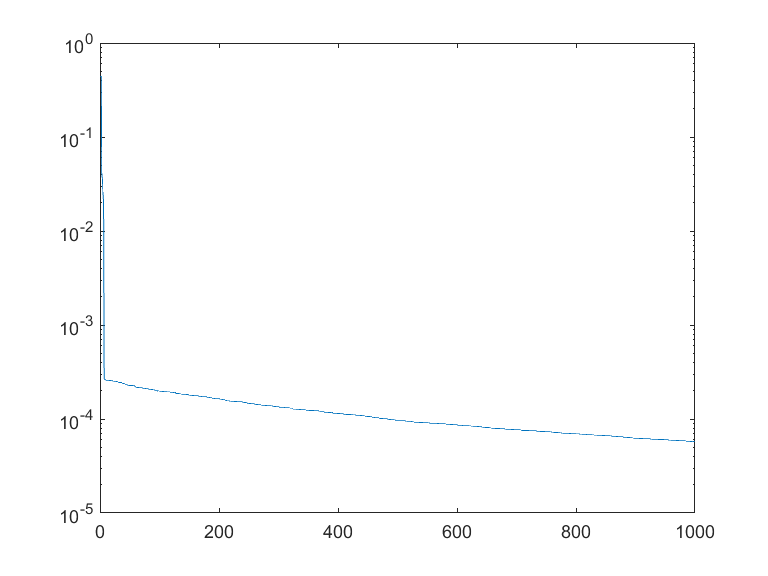
\includegraphics[width=0.8\textwidth]{example_error_plot}
    \caption{The error plot of a run with low badness.\label{fig:example_error_plot}}
  \end{figure}

  \begin{ex}
    \Cref{fig:example_error_plot_2} shows a error plot of an example with extremely high badness (0.913); and
    \cref{fig:example_error_plot_3} shows an example with medium badness (0.706).\footnote{Badness numbers will
    usually be quoted as proportions:- $ totalBadness/k $ where $ k $ is the number of iterations completed.}

    Note that in general a high badness corresponds to two characteristics of the error curve:
    \begin{itemize}
      \item A very long, shallow tail (i.e. for large $ x$-ordinates on the graph, $ \od{y}{x} \approx 0 $). This
            is particularly noticable in \cref{fig:example_error_plot_2}.
      \item A very `blocky' curve shape consisting of stretches of zero gradient interspersed with periods of
            extreme decline. This can be seen in \cref{fig:example_error_plot_3}.
    \end{itemize}
    The shallow tail corresponds to the fact that the algorithm decreases its step size according to the total
    badness (we shall discuss this in detail in a later section); the blockiness occurs because if it is `hard'
    for the algorithm to find a better candidate for the design then the error will remain constant over long
    stretches.

    Both of the graphs in this example were generated with $ (d,n,t) = (3,5,3) $, and it
    is known that there is no such design (see, e.g. the list given in \autocite[\S 6.16]{waldron2018});
    this explains why the asymptote of the error graph is non-zero (in this case, it
    appears to be $ \approx 26 $).
  \end{ex}

  \begin{figure}
    \centering
    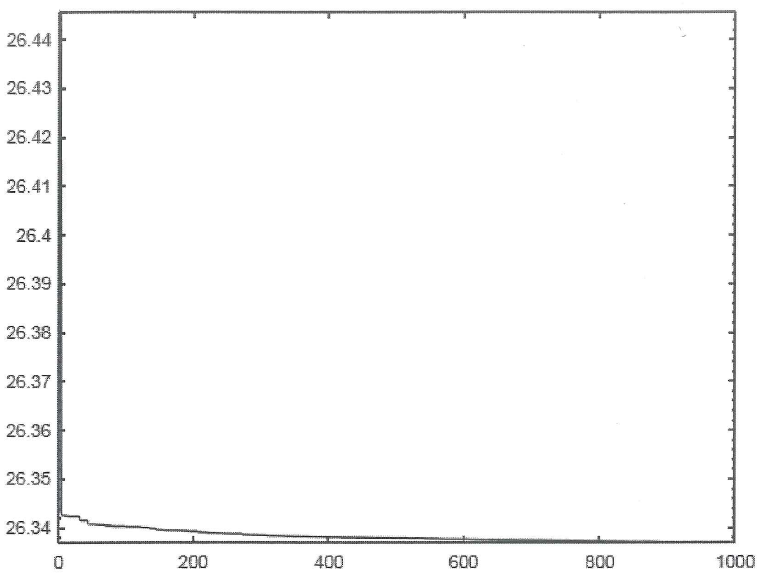
\includegraphics[width=0.8\textwidth]{example_error_plot_2}
    \caption{The error plot of a run with high badness.\label{fig:example_error_plot_2}}
  \end{figure}

  \begin{figure}
    \centering
    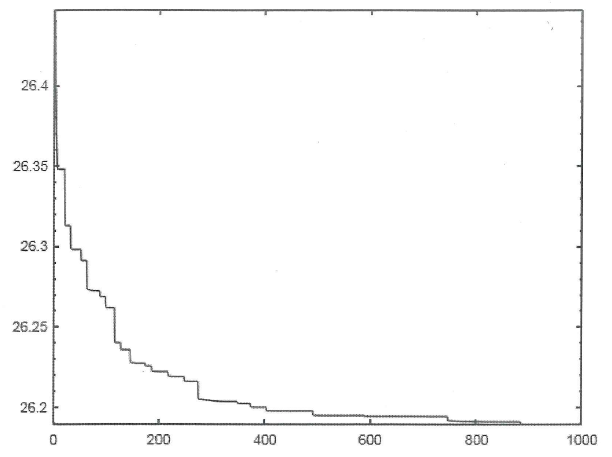
\includegraphics[width=0.8\textwidth]{example_error_plot_3}
    \caption{The error plot of a run with medium badness.\label{fig:example_error_plot_3}}
  \end{figure}

  \begin{table}
    \begin{threeparttable}
    \begin{tabularx}{\linewidth}{r|X|l}
      \textbf{Parameter} & \textbf{Description} & \textbf{Sane value}\\\hline
      $d$ & Dimension of the space to embed the design into.\\
      $n$ & Number of vectors in the design.\\
      $t$ & Parameter of the $ (t,t)$-design.\\
      $k$ & Number of iterations of the algorithm to run before returning.\\
      $s$ & Number of inital seed matrices to check. & \num{1e6}\\
      $b$ & Number of attempts at walking down the line of the gradient before falling back to looking at a ball. & \num{10}\\
      $ap$ & Number of times to run alternating projection on each iteration. & \num{10}\thinspace\tnote{a}\\
      $errorMultiplier$ & Scale factor for the walking distance at each iteration. & $1\times 10^{-4}$\thinspace\tnote{b}\\
      $fd$ & MATLAB file descriptor for progress output. & 1\thinspace\tnote{c}
    \end{tabularx}
    \begin{tablenotes}\footnotesize
      \item[a] According to \autocite[\S7.2.7]{tropp2004}, increasing $ ap $ beyond around \num{5000} does not significantly
               change the results obtained. However, note that in that thesis the projection algorithm itself is the convergence
               procedure (as opposed to the current project, in which a separate convergence step is performed). Thus we only
               need to run the projection a small number of times (and in fact larger numbers here will cause the Gram matrix
               to drift away from the line of descent towards a low value of $ \FP $).
      \item[b] If $ n $ is large, $ errorMultiplier $ should be made very small. For $ n \leq 4 $,
               $ errorMultiplier \approx \num{1e0} $ is OK; then decrease by powers of 10 from there. If
               the number is too large, it is more likely that the algorithm will go too far past the
               variety of $ (t,t)$-designs. If in doubt, set this small (especially if the badness proportion
               ends up high on test runs) and increase $ k $.
      \item[c] Set to `1' for console output; for file output set to \texttt{fopen('<filename>', 'w')}.
    \end{tablenotes}
    \end{threeparttable}
    \caption{Parameters for the \textproc{tightframe} method.\label{tab:tightframe_params}}
  \end{table}

  \begin{table}
    \begin{threeparttable}
    \begin{tabularx}{\linewidth}{r|X}
      \textbf{Return value} & \textbf{Description} \\\hline
      $result$ & A $ d \times n $ matrix consisting of $ n $ column vectors in $ \C^d $ which is putatively optimal
                 according to the error function.\\
      $errors$ & A $ k \times 1 $ matrix where the $ i$th value is the minimum error of the best design found by
                 iteration $ i $.\\
      $totalBadness$ & The total number of times that the algorithm failed to improve the estimate by walking
                       down the gradient. A more `efficient' run minimises $ totalBadness/k $ (where $ k $ is the
                       number of iterations).
    \end{tabularx}
    \end{threeparttable}
    \caption{Return values for the \textproc{tightframe} method.\label{tab:tightframe_returns}}
  \end{table}

  \subsection{The \texttt{runtf} script}
  The \textproc{tightframe} method is useful if the user wants to script the algorithm (e.g. try to run it for
  lots of values of $ n $ to find the minimal $ n $ such that a $ (t,t)$--design in $ \C^d $ exists). However,
  if the user does not need this power they will probably want to use the wrapper script in \texttt{runtf.m}.

  In order to change the design parameters (the same as those listed in \cref{tab:tightframe_params}, the user
  should change the first few lines of \texttt{runtf.m}; then the script (when run) will produce the following:
  \begin{itemize}
    \item The console output from \textproc{tightframe} in the console verbatim.
    \item A printout (to the default number of decimal places) of the returned $ d \times n $ matrix $ result $.
    \item A printout of the final error of that design (i.e. $ \FP_{\C^d,n,t}(result) $).
    \item A printout of the overall badness proportion $ totalBadness/k $.
    \item The parameters used for the generation of the design, together with the $ result $ matrix, the $ totalBadness $, and the list of $ errors $
          in the file \verb|tf_run_YYYY-MM-DD-HH-MM-SS.mat| (in the current directory).
    \item A plot of the best error over time (displayed on screen as a MATLAB figure).
  \end{itemize}

  \subsection{The \textproc{compute3Products} method}
  This method takes a single argument --- a $ d \times n $ matrix $ A $ --- and computes the set of all $ n^3 $ 3--products of the vectors of $ A $,
  sorted according to the MATLAB \textproc{sort} method.

  \subsection{The \texttt{generate.py} script}
  The purpose of this script, located in the top-level directory, is to take a directory of \texttt{.mat} files generated
  by the \texttt{runtf} method and produce a folder containing a nice HTML index of the generated designs.

  The script takes one required argument --- the directory in which to look for the \texttt{.mat} files. If the \texttt{-R}
  flag is specified, then the script will search recursively; otherwise it will search only the directory given and no subdirectories.
  For each \texttt{.mat} file it finds, the script will check whether it contains a variable called \texttt{result}. If it does,
  then it is copied to the output directory (default is \texttt{html/}, but this may be changed using the \texttt{-O} flag). An
  \texttt{index.html} file is also generated in the output directory containing a list of all the found designs, along with some
  parameters ($d$, $n$, $t$, and $k $ from \cref{tab:tightframe_params}, along with the error of the design found).

  If the flag \texttt{-e} is set, the script will attempt to connect to a running MATLAB instance; otherwise it will try to start
  MATLAB itself. If connection to an existing MATLAB instance is needed, the user should note that some user interaction is required:
  a command needs to be run in the MATLAB console and then the \Enter key needs to be pressed to make the script continue. The command
  needs only be run once for a given MATLAB instance.

  The up-to-date usage information for the script may be viewed by running \texttt{python generate.py -h}.

  \section{Mathematical background}
  Let $ \scrH $ be a finite-dimensional Hilbert space of dimension $ d $ (so, as a vector space,
  $ \scrH \simeq K^d $ for some field $ K $), and let $ \scrS_\scrH(n) $ be the set of finite
  sequences of $ n $ elements of $ V $ with unit norm:
  \begin{displaymath}
    \scrS_\scrH(n) := \{ (v_i)_{i = 1}^n : \forall_i (v_i \in V \text{ and } \norm{v_i} = 1) \}.
  \end{displaymath}

  Suppose $ S $ is the unit sphere in $ \scrH $, let $ \sigma $ be a normalised measure
  on $ S $, and suppose we have picked an orthonormal basis $ (w_i)_{i = 1}^d $ on $ \scrH $.
  Let $ \pi $ be the projection map from $ \scrH $ onto the subspace spanned by $ w_1 $,
  and for each $ t \in \N $ define the \df{bound weighting} $ c_t(\scrH) $ to be the (real) quantity
  \begin{displaymath}
    c_t(\scrH) = \left(\rint_S \norm{\pi v}^{2t} \dif{\sigma(v)}\right)^{-1}.
  \end{displaymath}
  (Remark: the quantity $ c_t(\scrH) $ is independent of the choice of basis.)

  Finally, define the functions $ \FP_{\scrH,n,t} : \scrS_\scrH(n) \to \R $ by the rule
  \begin{equation}\label{eqn:fp}
    \FP_{\scrH,n,t} : (v_i)_{i = 1}^n \mapsto
          c_t(\scrH) \sum_{i = 1}^n \sum_{j = 1}^n \abs{\inp{v_i, v_j}}^{2t}
            - n^2.
  \end{equation}
  The value of $ \FP $ for a given design is called the \textit{error} of that design.

  Define the set $ \SD_\scrH(n,t) := \FP_{\scrH,n,t}^{-1}(0) $; the elements of this set
  are called \df{spherical $ (t,t)$-designs} of order $ n $, embedded in $ \scrH $. (These
  designs obviously also depend on $ \sigma $, the spherical measure --- but usually this
  comes naturally with $ \scrH $.)

  If $ \scrH = \R^d $ or $ \scrH = \C^d $ (with the usual inner product and with $ \sigma $
  the normalised surface area measure of the sphere) then one can precalculate the following
  values \autocite[122]{waldron2018}:-
  \begin{displaymath}
    c_t(\R^d) = \frac{d(d+2)\cdots(d+ 2(t-1))}{1\cdot3\cdot5\cdots(2t-1)},
    \qquad
    c_t(\C^d) = \binom{d+t-1}{t}.
  \end{displaymath}

  The data of a design may be summarised by a $ d \times n $ matrix $ V $ whose columns form
  the $ n $ column vectors of the design with respect to the basis $ (w_i) $. A frequently
  more useful representation, however, is the $ n \times n $ \df{Gram matrix} of the design:
  \begin{displaymath}
    \Gamma((v_i)_{i=1}^d) = [V^* V] = [\inp{v_j,v_i}_{i,j}].
  \end{displaymath}

  It can be shown that the Gram matrix $ \Gamma $ has the following properties:
  \begin{enumerate}[label=(G\arabic*)]\label{pg:gram_properties}
    \item $ \Gamma $ is Hermitian;
    \item $ \Gamma $ has unit diagonal;
    \item $ \Gamma $ is positive definite;
    \item $ \Gamma $ has rank $ d $;
    \item $ \Gamma $ has trace $ n $.
  \end{enumerate}
  Note that (1) and (2) are conditions on the \emph{entries} of $ \Gamma $, while (3), (4), and (5) are conditions
  on the \emph{spectrum} of $ \Gamma $.

  We may also find the gradient of $ \FP_{\scrH,n,t} $ with respect to the entries of the Gram
  matrix: we may rewrite $ \FP $ in terms of $ \Gamma $ as
  \begin{displaymath}
    \FP_(\scrH,n,t) : \Gamma \mapsto c_t(\scrH) \sum_{i = 1}^n \sum_{j = 1}^n \abs{\Gamma_{j,i}}^{2t} - n^2
  \end{displaymath}
  and taking the partial derivatives of this, we obtain
  \begin{displaymath}
    \pd{\FP}{\Gamma_{i,j}} = t\thinspace c_t(\scrH)\thinspace \abs{\Gamma_{i,j}}^{2(t-1)} \thinspace \overline{\Gamma_{i,j}};
  \end{displaymath}
  thus to decrease the frame potential we must perturb the Gram matrix in the direction $ -\nabla \FP $
  where $ (\nabla \FP)_{i,j} = \pd{\FP}{\Gamma_{i,j}} $.

  \section{Algorithms implemented}
  In this section we will give pseudocode for the operations that are implemented by this
  package, along with explaining various design choices and limitations of the approach.

  \subsection{The high-level method}
  The high-level method is implemented in \textproc{tightframe}, listed in \cref{alg:high_level}.
  The algorithm as described here does not take the $ fd $ parameter listed in \cref{tab:tightframe_params},
  as this is only used to print status updates.

  We begin by choosing a good starting Gram matrix (line \ref{line:seed}). We generate $ s $ different matrices
  with the properties (G1)--(G5) (the `seed' matrices), and pick the one which minimises the potential function
  to begin the iteration with.

  The actual iteration begins on line \ref{line:tf_iter}; the variable $ badCount $ holds the number of iterations
  since the current best matrix $ A $ was found, and if $ badCount < b $ we attempt to walk down the gradient
  a small random amount. The mean distance to walk, $ \frac{error \times errorMultiplier}{totalBadness + 1} $,
  is proportional to $ error $ (so when we are `close' the distance we walk decreases), and inversely proportional
  to $ totalBadness $ (so if we keep failing to find a good choice the step size decreases).

  If $ badCount $ exceeds the parameter $ b $, we stop trying to walk down the gradient and instead we pick
  random matrices from the `ball' $ B $ around $ A $ of mean distance $ error\times errorMultiplier$. The idea here
  is that if the badCount is high then we keep trying and failing to walk along the line of steepest descent
  towards the variety of $ (t,t)$--designs, and so the path of steepest descent must be twisting sharply away
  from the path it has been taking (\cref{fig:badness_illustration}). The amount we try to walk along the path
  of steepest descent keeps decreasing as the badness (i.e. failure rate) increases, but if the path is very
  twisty then this permanently makes the walk distance tiny and so the convergence rate will become very slow.
  Instead, if the $badCount$ becomes large, we instead look at the ball $ B $ (dotted blue) of (relatively) large radius, in
  the hope that we will hit upon the path of steepest descent again after it has rounded the corner, we will tend
  to skip part of the path and rejoin it on a straighter section (the dotted arrow on the figure) without having to
  drop our rate of walking too far. This can be seen in the console output: long runs of \texttt{*** Better found, ...} tend to
  accompany very small decreases of the error, while occasional blocks of \texttt{Nothing better}  tend to be followed by a sharp decrease
  in the error. In order to take advantage of this, a healthy \texttt{badnessProportion} should be around 0.7.

  \begin{figure}
    \centering
    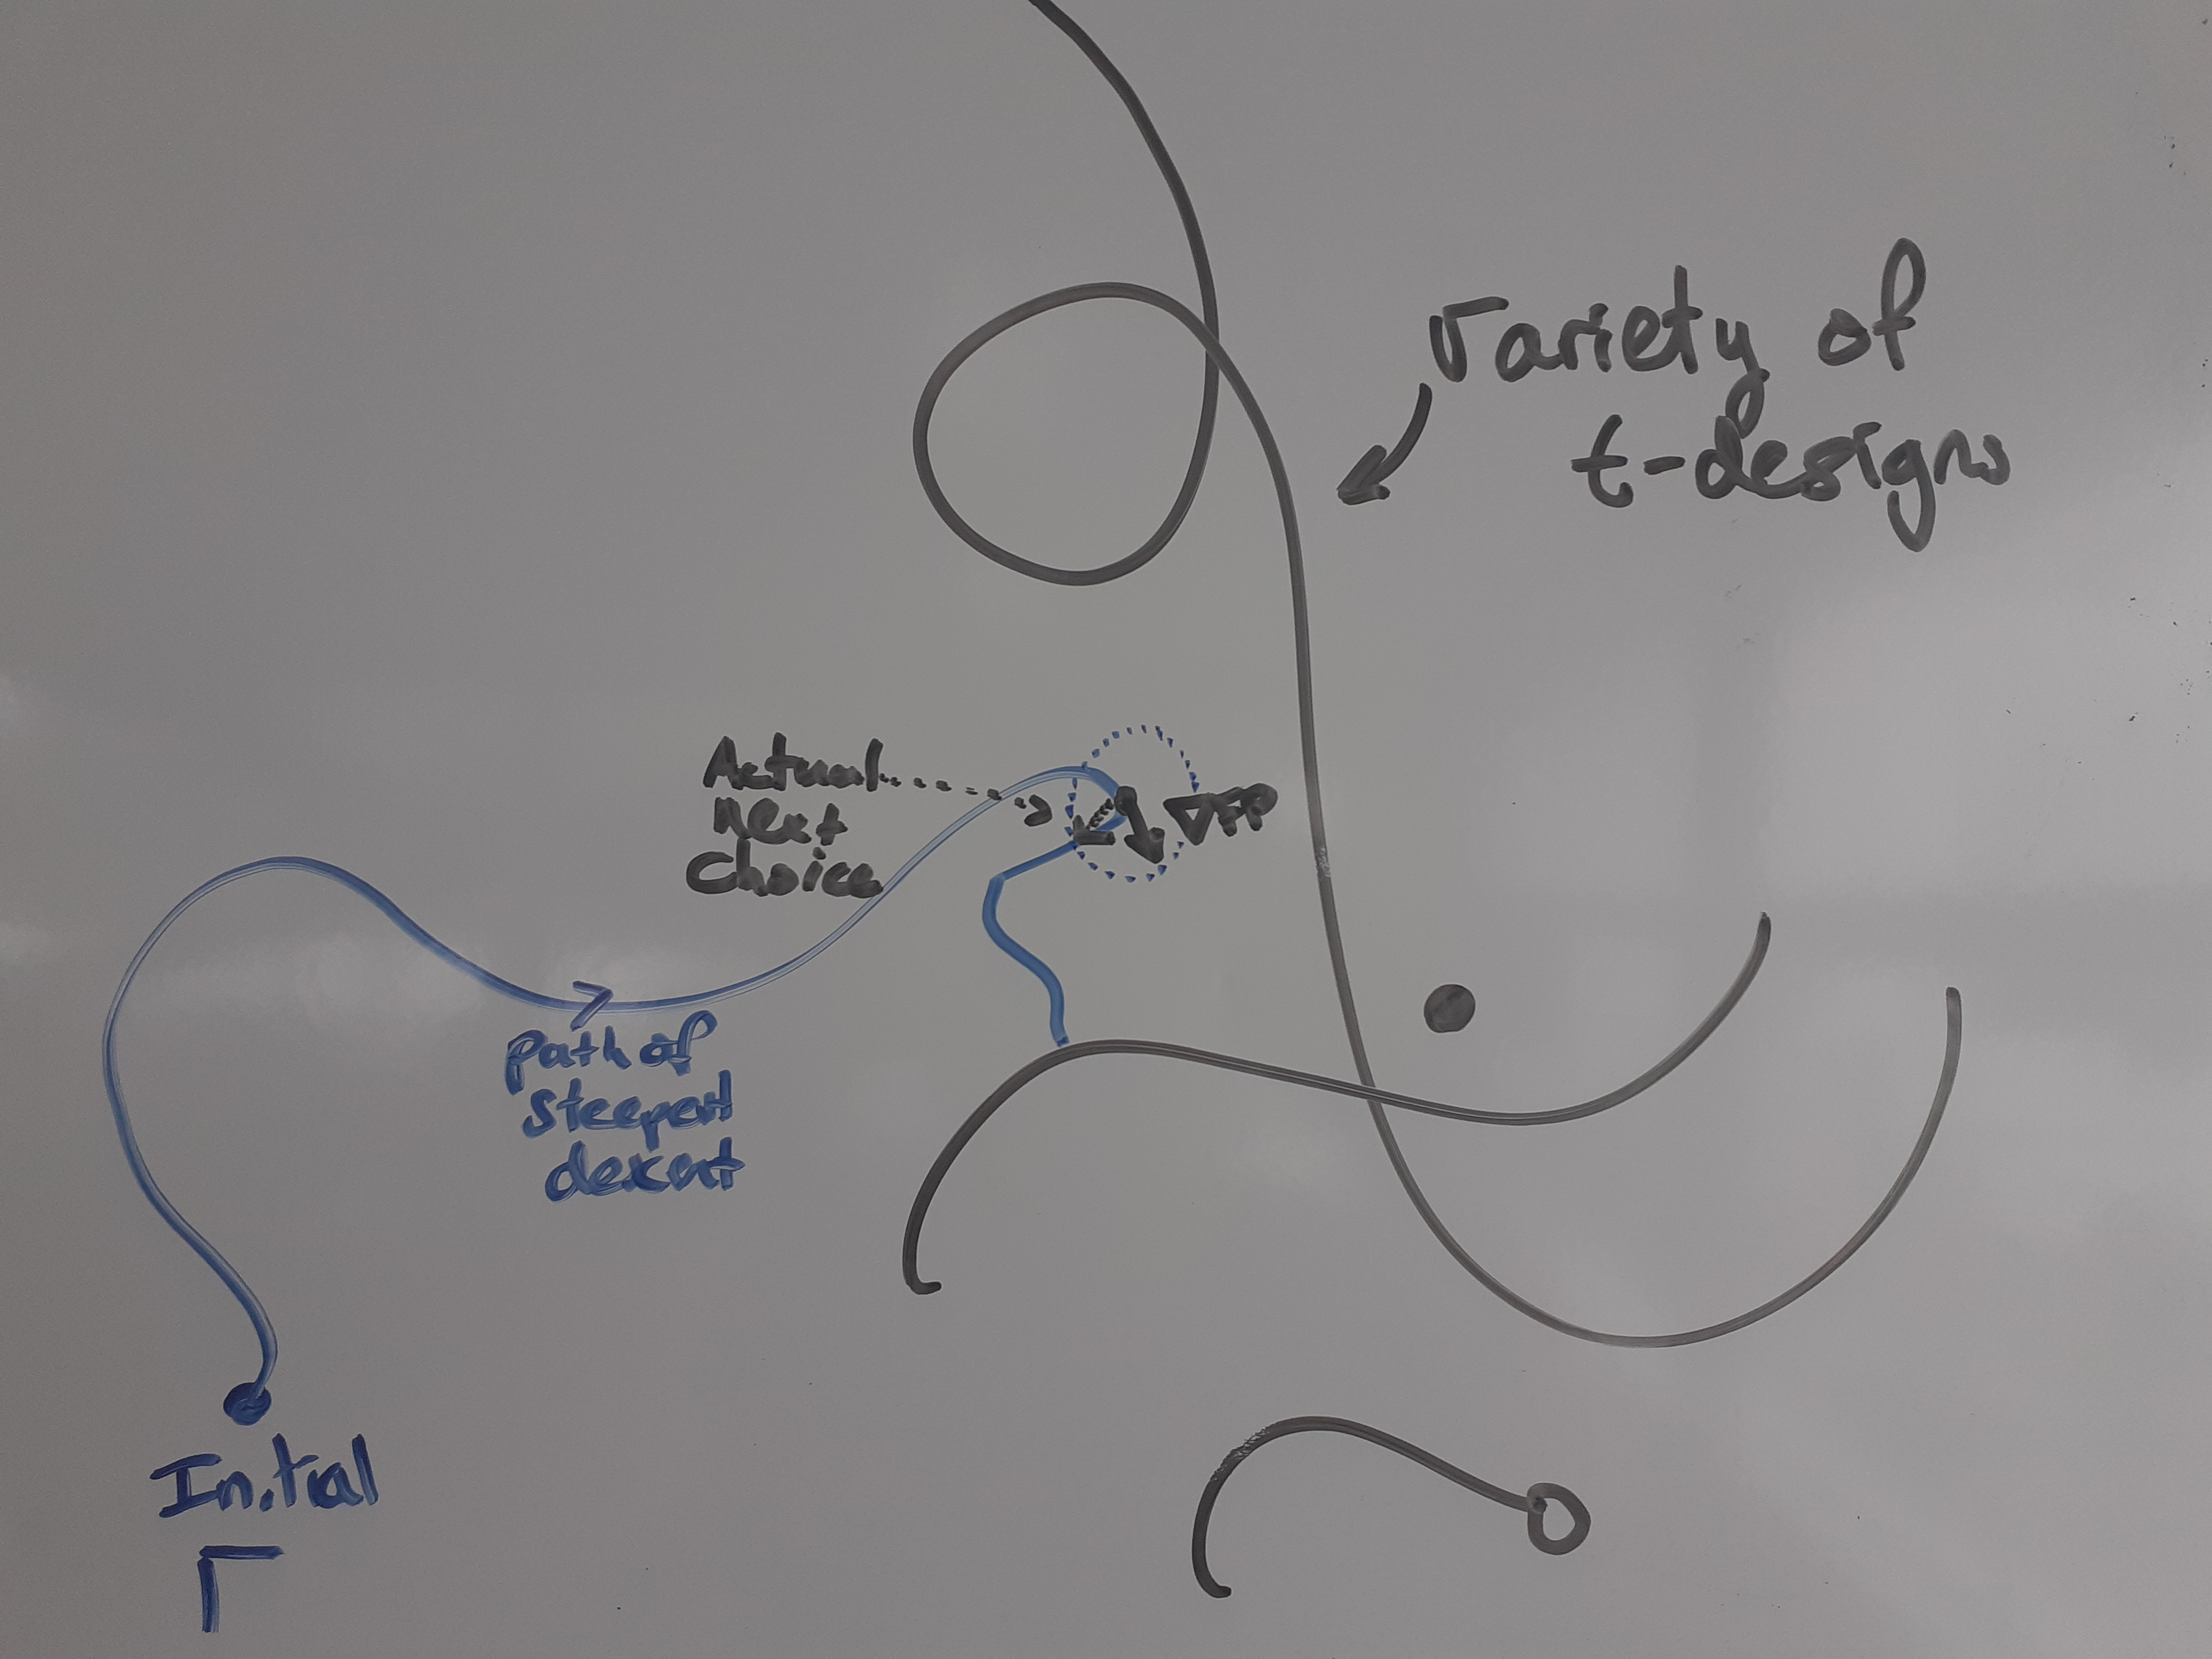
\includegraphics[width=0.8\textwidth]{badness_illustration}
    \caption{An intuitive depiction of the way counting `badness' allows the algorithm to skip twists in the path of steepest descent.\label{fig:badness_illustration}}
  \end{figure}


  In either case we have picked a new random candidate for Gram matrix near $ A $; we call it $ A_\mathrm{new} $.
  Since the randomisation process does not guarantee that $ A_\mathrm{new} $ is Hermitian, we project it onto
  the space of Hermitian matrices (line \ref{line:make_hermitian}); then we attempt to project it onto the space
  of matrices satisfying the properties (G1)--(G5). This is done by the method \textproc{alternatingProjection}
  described below; \textproc{tightframe} passes into this method the parameter $ ap $ to modify the accuracy
  of the alternating projection algorithm, as well as the matrix $ A_\mathrm{new} $ and the desired rank $ d $.

  Finally, we compute the error of the resulting matrix; if it is lower than the current best we set the $ badCount $
  back to zero; otherwise we increase both $ totalBadness $ and $ badCount $.

  When the loop is done, we are left with a Gram matrix $ A $ satisfying (G1)--(G5). The final diagonalisation process
  undoes the map $ V \mapsto \Gamma = V*V $ which produces the Gram matrix from the initial vectors. The resulting
  $ n \times n $ matrix will have $ n - d $ zero rows (by consideration of the rank of $ A $) and so we project down
  to $ \C^d $ in the natural way to produce the final matrix $ result $ which is returned.

  \begin{algorithm}
    \caption{The high-level method}\label{alg:high_level}
    \begin{algorithmic}[1]
      \Procedure{tightframe}{$d,n,t,k,s,b,ap,errorMultiplier$}
        \State Find a good starting matrix $ A $ which satisfies properties (G1)--(G5) by checking $ s $ different
               matrices, $ A_1,...,A_s $ and calculating $\FP_{\C^d,n,t}(A_i)$ for each. \label{line:seed}
        \State $ error \gets \FP_{\C^d,n,t}(A) $
        \State $ errors \gets [] $
        \State $ badCount \gets 0 $
        \State $ totalBadness \gets 0 $
        \State $ h \gets 1 $
        \While{$ h \leq k $} \label{line:tf_iter}
          \State Append $ error $ to $ errors $.
          \If{$badCount < b $}
            \State $ \delta \gets $ a random positive value near $ \frac{error \times errorMultiplier}{totalBadness + 1} $
            \State $ A_{\mathrm{new}} \gets A - \delta \nabla\FP_{\C^d,n,t}(A) $
          \Else
            \State $ \Delta \gets $ an $ n \times n $ matrix of random values near $ (error \times errorMultiplier) $
            \State $ A_{\mathrm{new}} \gets A + \Delta $
          \EndIf
          \State $ A_{\mathrm{new}} \gets \frac{A_{\mathrm{new}} + A_{\mathrm{new}}^*}{2} $\label{line:make_hermitian}
          \State Project $ A_{\mathrm{new}} $ onto the space of matrices satisfying (G1)-(G5).
          \State $ error_\mathrm{new} \gets \FP_{\C^d,n,t}(A_{\mathrm{new}}) $

          \If{$error_\mathrm{new} < error$}
            \State $ A \gets A_\mathrm{new} $
            \State $ error \gets error_\mathrm{new} $
            \State $ badCount \gets 0 $
          \Else
            \State $ badCount \gets badCount + 1 $
            \State $ totalBadness \gets totalBadness + 1 $
          \EndIf
        \EndWhile

        \State $ U \gets $ the $ n \times n $ matrix of eigenvectors of $ A $
        \State $ D \gets $ the diagonal matrix of corresponding eigenvalues
        \State $ result \gets D^{1/2}U $
        \State Delete the zero rows of $ result $, producing a $ d \times n $ matrix (by rank of $ A $).
        \State Return $ (result, errors, totalBadness) $.
      \EndProcedure
    \end{algorithmic}
  \end{algorithm}

  \section{Further work to be done}
  \begin{itemize}
    \item Allow users to pass in an error function to be minimised.
    \item Add support for real designs.
    \item Save all generated designs in a database.
    \item Implement an algorithm to partition generated designs into unitary equivalence classes.
  \end{itemize}

  \printbibliography
\end{document}
